\documentclass[practice]{ijdc-v9} 

\usepackage[style=apa]{biblatex}
\addbibresource{my.bib}
\DeclareLanguageMapping{british}{british-apa}

\title{YesWorkflow: A User-Oriented, Language-Independent Tool for Recovering Workflow Structure, Provenance, and Semantics from Scripts}

\author{tianhong, tim, bertram,}
\affil{Digital Curation Centre}
\correspondence{xyz company Email: \email{a.ball@ukoln.ac.uk}}

\received{18 January 2015}
\revised{19 January 2015}
\accepted{1 January 2015}

\begin{document}

\maketitle

\section{Abstract}
Abstract Abstract   Abstract  
 
\section{Introduction and Motivation}

A scientific workflow\autocite{apa6ed} is a formal description of a process for accomplishing a scientific task, usually expressed in terms of tasks and their (dataflow) dependencies. Scientific workflows can include steps for the acquisition, integration, reduction, analysis, visualization, sharing, and curation of scientific data.  Scientific workflow management systems (SWfMSs) provide controlled environments for computational scientists to construct complex computational pipelines from modular buildings blocks. Advantages offered by SWfMSs include the intuitive rendering of the workflows as a directed graph, showing the computational steps and the dataflow between them, and the construction and visualization interfaces that they provide, which enable scientists to review, revise, and share their workflows as ?schemas? or schematic diagrams that are distinct from any specific workflow execution. In addition, many SWfMSs (e.g.: Kepler [CITE], Taverna [CITE], Pegasus [CITE], VisTrails [CITE], and Galaxy [CITE]) have been instrumented with runtime, or retrospective provenance capture and management capabilities. The provenance traces generated from workflow runs have been shown to be useful in a number of settings, helping scientists (i) examine the sequence of steps that led to a result; (ii) identify which inputs were used; (iii) interpret and understand outputs; and (iv) verify that the steps were performed according to acceptable procedures. 

\subsection{heading 1.1}

\paragraph{ddd}

\subparagraph{ddddddd}

\section{System Architecture}

Figure example:   Figure~\ref{fig:start-paper}.

\begin{figure}[h]
    \centering
    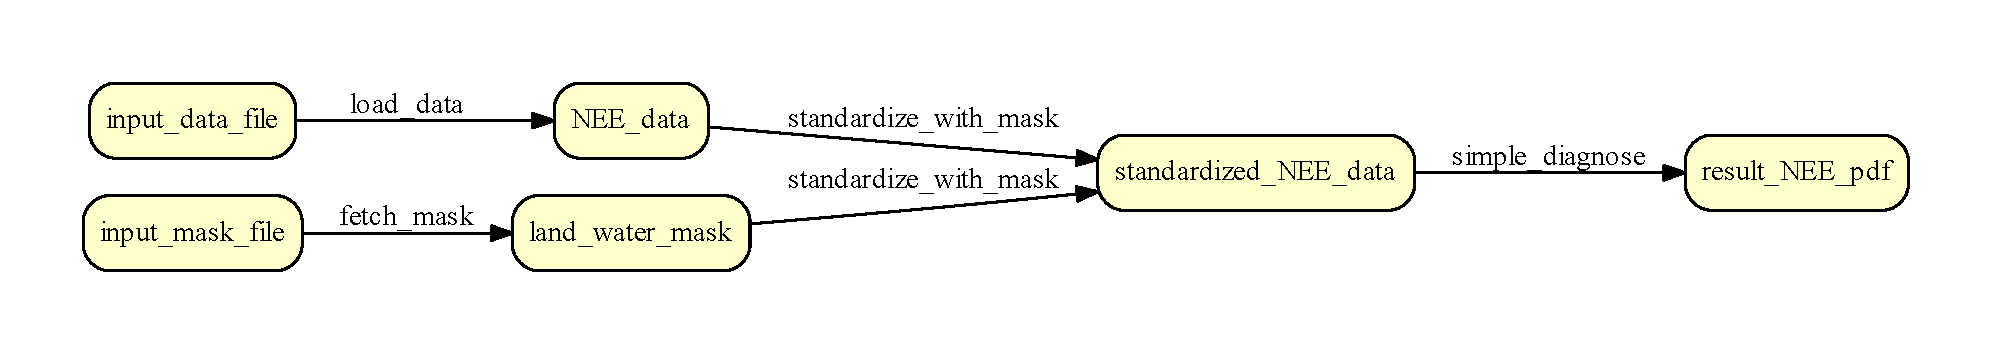
\includegraphics[width=3.0in, height=2in]{image1.pdf}
    \caption{Caption for figure}
    \label{fig:start-paper}
\end{figure}


\begin{table}
\caption{Papers and articles published in the IJDC in 2008 and 2009.} 
\label{tab:issues} 
\centering\small 
\begin{tabular}{|r|r|}
\hline
$n$&$n!$\\
\hline
1&1\\
2&2\\
3&6\\
4&24\\
5&120\\
6&720\\
7&5040\\
8&40320\\
9&362880\\
10&3628800\\
\hline
\end{tabular}\end{table}



\begin{itemize}
\item\textsf{atbegshi} is used for switching geometry between pages.
\item Tables in your document must be formatted according to the design principles promoted and supported by the \textsf{booktabs} package.
\item\textsf{caption} is used to format the figure and table captions.
\item\textsf{etoolbox} is used behind the scenes for patching commands.
\item\textsf{footmisc} is used to format the footnotes.
\item\textsf{titlesec} is used to format the section headings.
\end{itemize}





\section{Acknowledgements}

Any acknowledgements should be placed in a section immediately before the references.\nocite{*}

\printbibliography
%\bibliography{my.bib}

\end{document}